\parindent=0em
\subsection{Hololens 2}
\label{HoloLens2Dispositivo}
\noindent

Las \textit{HoloLens 2} (figura~\ref{fig:vistasHoloLens2}) son un casco desarrollado por \textit{Microsoft} que salió al mercado en 2019. Es un dispositivo dotado de tecnología de \textit{eye tracking} y \textit{hand tracking} capaz de detectar las dos manos, esto añade un extra de inmersión a la experiencia y de comodidad ya que no se necesitan mandos para manejarlo y se pueden tener las manos libres. Respecto a los sensores, goza de acelerómetro, giroscopio y magnetómetro para medir la velocidad, orientación y fuerzas gravitacionales del dispositivo.\\


\begin{figure}[htbp]
\centering
    \hspace{-4mm}
    \begin{minipage}{0.5\textwidth}
        \centering
        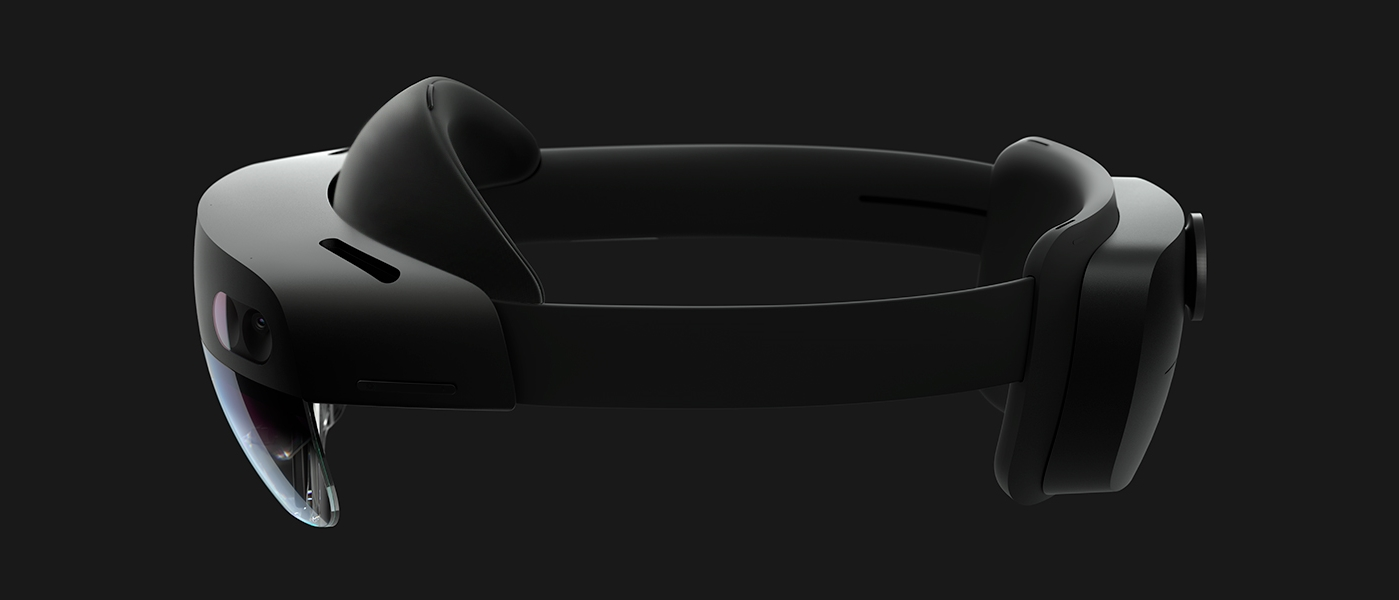
\includegraphics[scale=0.2]{Images/Estado del arte/hololens2_2.jpeg}\\
        (a) Vista lateral.
    \end{minipage}
    \begin{minipage}{0.5\textwidth}
        \centering
        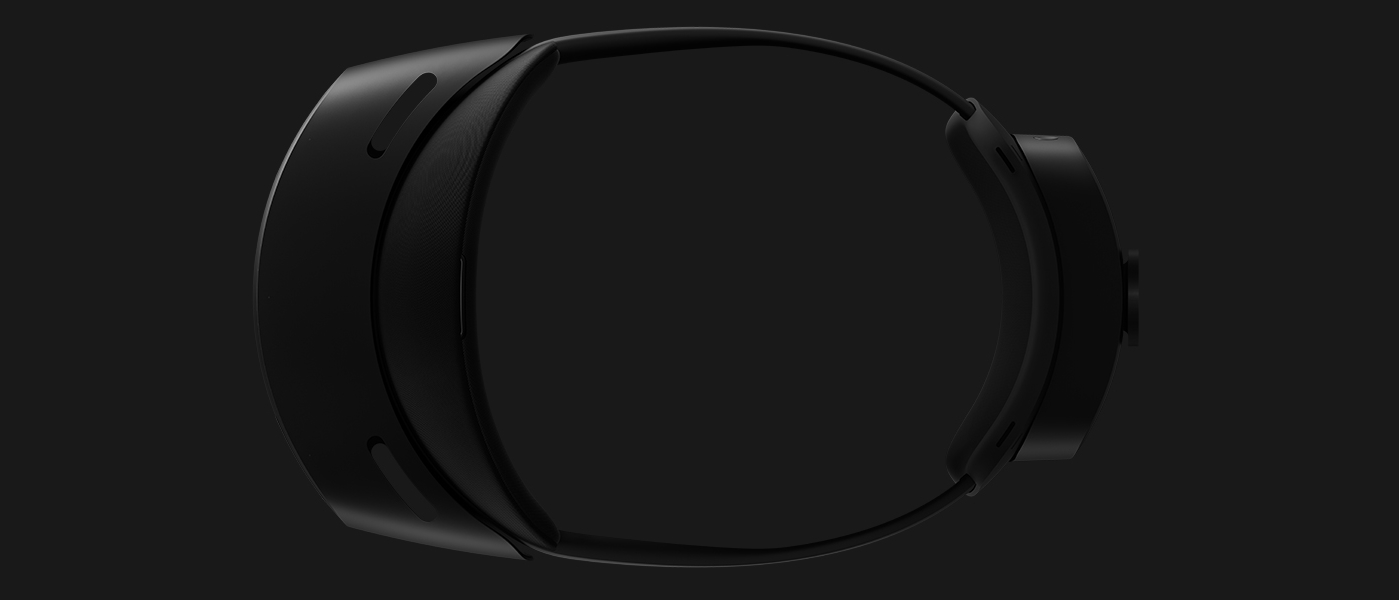
\includegraphics[scale=0.2]{Images/Estado del arte/hololens2_3.jpeg}\\
       (b) Vista superior.
    \end{minipage}\\
    \caption{Vistas de las Microsoft HoloLens 2\textsuperscript{\ref{hololens2footer}}.}
    \label{fig:vistasHoloLens2}
\end{figure}


Las \textit{Hololens 2} funcionan de forma independiente ya que tienen integrado su propio procesador y utilizan una batería recargable con una autonomía de entre 2 y 3 horas, además, permiten capturar el movimiento y los giros del usuario gracias a su control de \textit{6DoF}. Por otra parte, respecto a la conectividad, este \textit{HMD} tiene \textit{WiFi}, \textit{bluetooth} y permite conexiones mediante un \textit{USB} tipo C. Por ejemplo, se puede utilizar la conexión \textit{WiFi} para navegar por internet (a través del navegador \textit{Microsoft Edge} incorporado en las gafas) o para conectarse a reuniones en línea con otros usuarios de las mismas gafas.\\

Del mismo modo, este casco  está diseñado con un sistema ergonómico de tal forma que no hay necesidad de quitarse las gafas, ya que se puede colocar directamente sobre ellas (figura~\ref{fig:hololensErgonomicas}).\\


\begin{figure}[H]
    \centering
    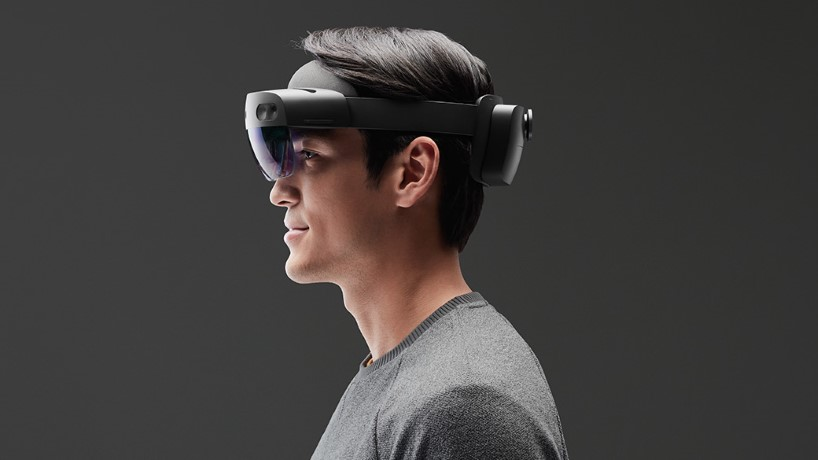
\includegraphics[scale=0.35]{Images/Estado del arte/hololens2_1.jpeg}
     \caption{Diseño ergonómico del dispositivo\textsuperscript{\ref{hololens2footer}}.
  }
  \label{fig:hololensErgonomicas}
\end{figure}


Para finalizar, este \textit{HMD} tiene un \textit{FOV} de 43º, una resolución de 2.048×1.080 píxeles por ojo (4.096x1.080 en combinación) y una \textit{IPD} que se ajusta automáticamente según la posición de los ojos que es detectada por un sensor \textit{IPD}, asimismo, tiene un sensor de~1~Megapíxel de profundidad \textit{ToF} (del inglés Time of Flight, calcula distancias entre objetos en función a la distancia que tarda la emisión y recepción de un haz de luz infrarrojo) y un peso de 566 gramos.  


%https://www.microsoft.com/es-es/hololens/hardware


